\section{Example: what it looks like if you compile like normal}
\label{sec:compile-like-normal}

If one would skip the \sysname pipeline and directly compile the \LaTeX{} from the example in \S\ref{sec:example} (\ie using pdflatex, bibtex), it produces placeholders for the unavailable expincludes:

\vspace{0.2cm}
% %%%%%%%%%%%%%%%%%%%%%%%%%%%%%%%%%%%%%%%%%%%%%%%%%%%%%%%%%
% NOTE: the underneath LaTeX does not have any \expinclude... commands, because it is just to showcase what would happen if one would not execute the CodeBind pipeline beforehand. If we would use expincludes with either incorrect experiment names or incorrect filenames here, the pipeline would throw an error when going over this section.
\begin{mdframed}[style=annotex]

Under max-min fairness, the addition of flows to the network can \emph{increase} the throughput of some flows.

To demonstrate this, we use a simple topology of three nodes with two directed edges:
the edge from A to B has a capacity of 1 unit,
and the the edge from B to C has a capacity of 1 unit.

In the first experiment, we start the following flows: one from A to B (path is A$\rightarrow$B), one from B to C (path is B$\rightarrow$C), and one from A to C (path is A$\rightarrow$B$\rightarrow$C).
This results in a max-min fair allocation of \textbf{\textcolor{red}{[\texttt{X}]}}, \textbf{\textcolor{red}{[\texttt{X}]}} and \textbf{\textcolor{red}{[\texttt{X}]}} for each type respectively.

\begin{center}
% Source file: figures/topology-example.drawio

\includegraphics[width=3cm]{figures/topology-example.pdf}
\end{center}

However, say we increase the number of flows from A to B. What would happen to the flow from B to C? In the second experiment, as before we start one flow from B to C and one flow from A to C. We vary the number of flows from A to B between 1 and 4. The addition of extra flows from A to B results in the flow from A to C being bottlenecked there, resulting in the flow from B to C being allocated more.

\begin{center}
\includegraphics[width=4.7cm]{example-image-a}
\end{center}

\end{mdframed}
% %%%%%%%%%%%%%%%%%%%%%%%%%%%%%%%%%%%%%%%%%%%%%%%%%%%%%%%%%

%%%%%%%%%%%%%%%%%%%%%%%%%%%%%%%%%%%%%%%%%%%%
%%%%%%%%%%%%%%%%%%%%%%%%%%%%%%%%%%%%%%%%%%%%
%%%%%%%%%%%%%%%%%%%%%%%%%%%%%%%%%%%%%%%%%%%%
%%%%%%%%%%%%%%%%%%%%%%%%%%%%%%%%%%%%%%%%%%%%
%%%%%%%%%%%%%%%%%%%%%%%%%%%%%%%%%%%%%%%%%%%%

\section{Publication venue reproducibility pipeline}
\label{appendix:reproducibility}

An overview of the publication venue reproducibility pipeline is depicted in Fig.~\ref{fig:venue-reproducibility-pipeline}. The authors supply the two artifacts, and the CI/CD pipeline spins up a fresh start container, clones the code base into it, and executes the \textit{setup\_env.sh} and \textit{reproduce.sh} scripts. Venue should store the container both after successful completion of \textit{setup\_env.sh} and after \textit{reproduce.sh} to safeguard against \eg dependency evolution or fallout. Although the first container should have the entire environment setup, the second container is stored in the eventuality of there mistakenly being an external dependency being retrieved by the \textit{reproduce.sh} script. The generated PDF would be compared against the submitted PDF for any differences, and a report could be generated as a result for both authors and reviewers (see Fig.~\ref{fig:reproducibility-checker} and \ref{fig:paper-pdf-delta}).

\parab{Code base pointer and checksum.} We define one extra command: \texttt{\textbackslash expcodechecksum\{\}} prints the code checksum. It import the value from the \textit{code-checksum.txt} file within the paper \LaTeX{} folder. The checksum of the code base is either (a) if it was supplied as a single file archive, its (SHA-256) hash, or (b) if it is a git repository, its git commit hash. Authors first finalize their code base and determine the checksum. Afterwards, they run their code one more time with the correct code checksum to generate the PDF to submit -- it is never committed to the code base. The code checksum must be set to zeroes in the code base (to prevent a cyclic dependency). The reproducibility submission system would similarly calculate or retrieve the checksum from the submitted code base, and insert it before starting the code base execution.

The authors must place the following piece of \LaTeX{} in their paper:

\vspace{0.2cm}
\begin{mdframed}[style=annotex]
\begin{verbatim}
This paper is written using CodeBind.
\url{https://venue.com/year/paper-name}
Code checksum: \expcodechecksum{}
\end{verbatim}
\end{mdframed}

\noindent If the submission system permits authors to supply supplemental archives, the URL can potentially be left out while the paper is under submission though must be included in the camera-ready.

\begin{figure}
    % Source file: figures/venue-reproducibility-pipeline.key
    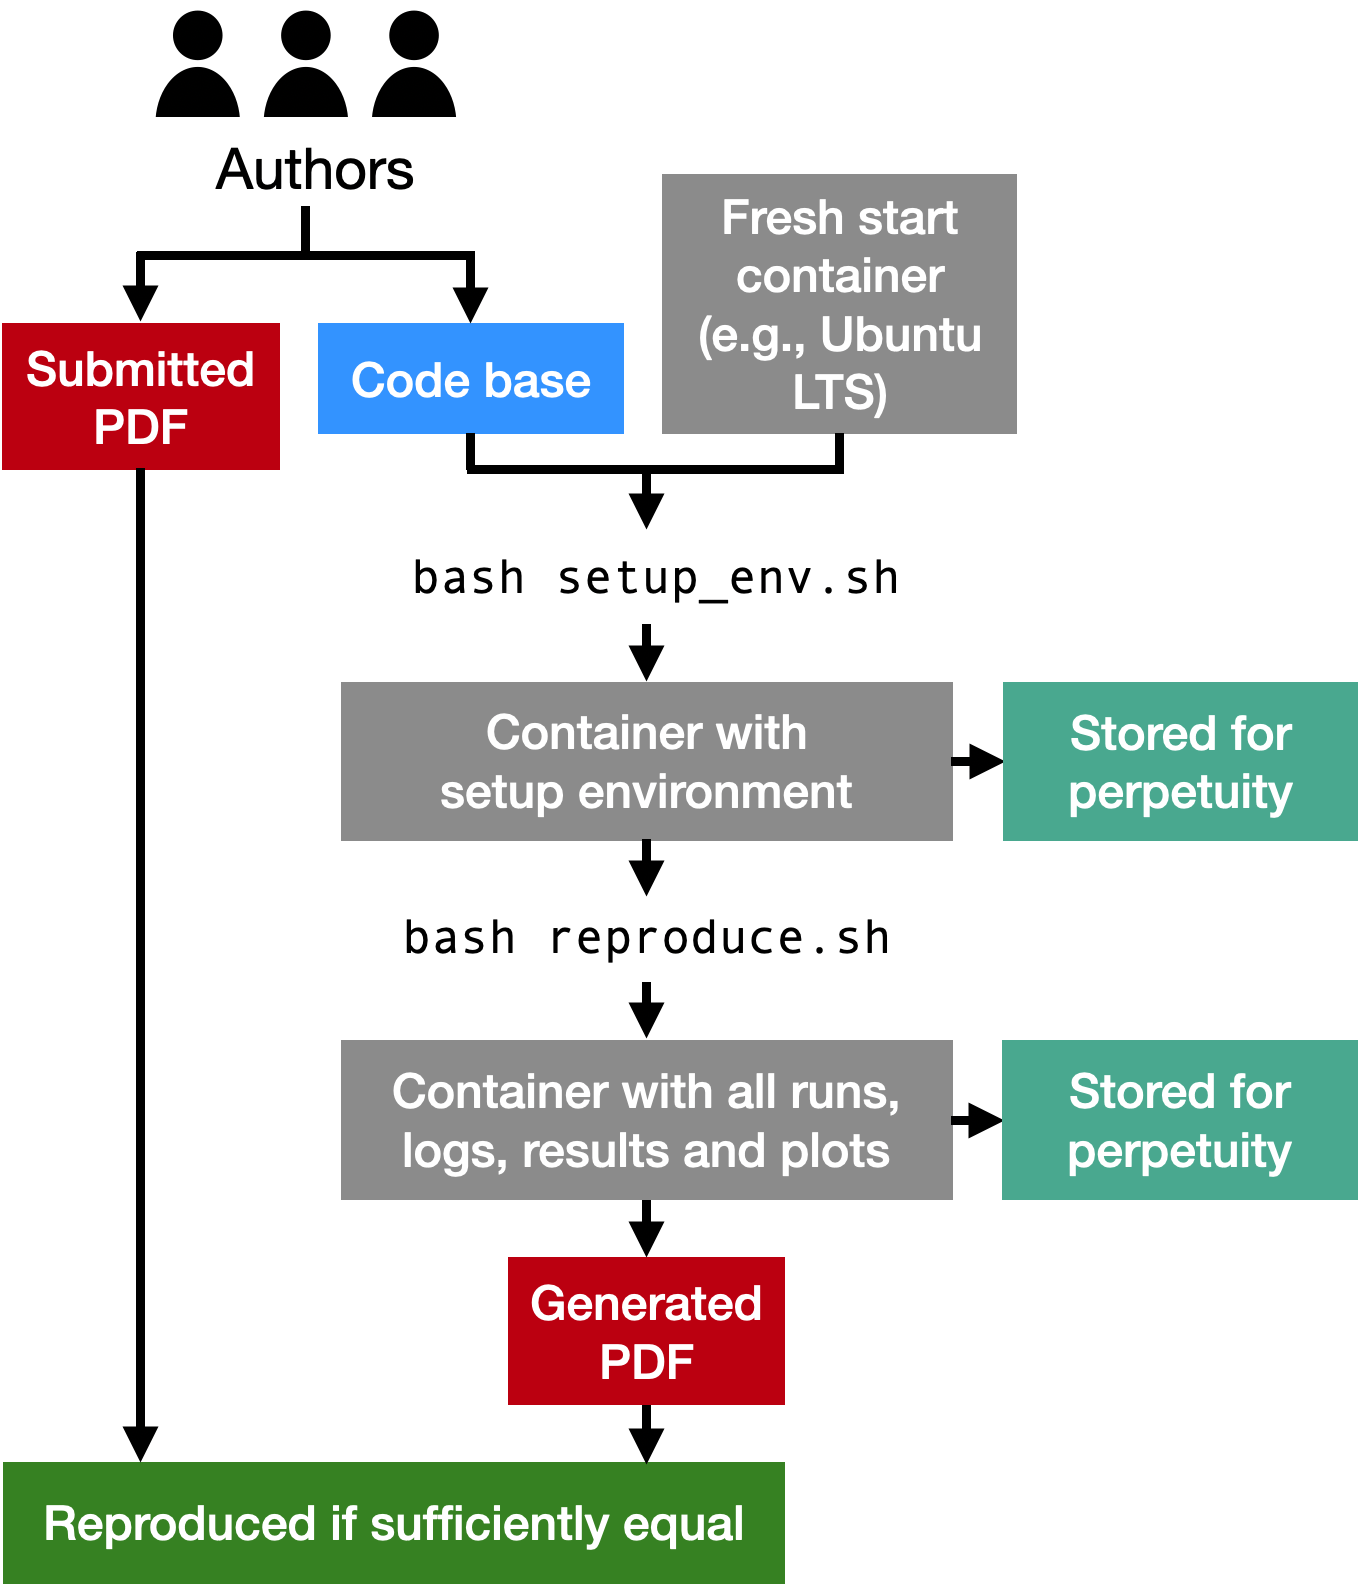
\includegraphics[width=0.48\textwidth]{figures/venue-reproducibility-pipeline.png}
    \caption{Overview of a pipeline a publication venue could use to enforce reproducibility.}
    \label{fig:venue-reproducibility-pipeline}
\end{figure}

\begin{figure}
    % Source file: figures/reproducibility-checker.key
    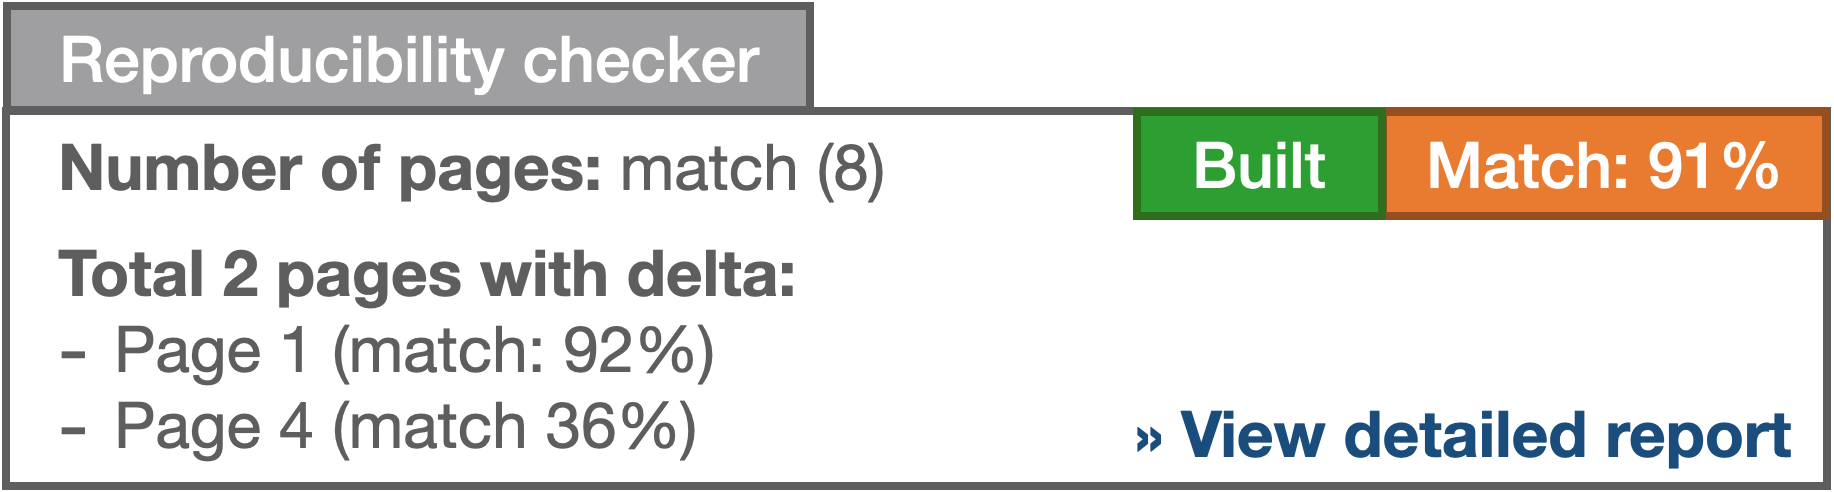
\includegraphics[width=0.48\textwidth]{figures/reproducibility-checker.png}
    \caption{Similar to the format checker in HotCRP, we propose the reproducibility checker (mock-up).}
    \label{fig:reproducibility-checker}
\end{figure}

\begin{figure}
    % Source file: figures/paper-pdf-delta.drawio
    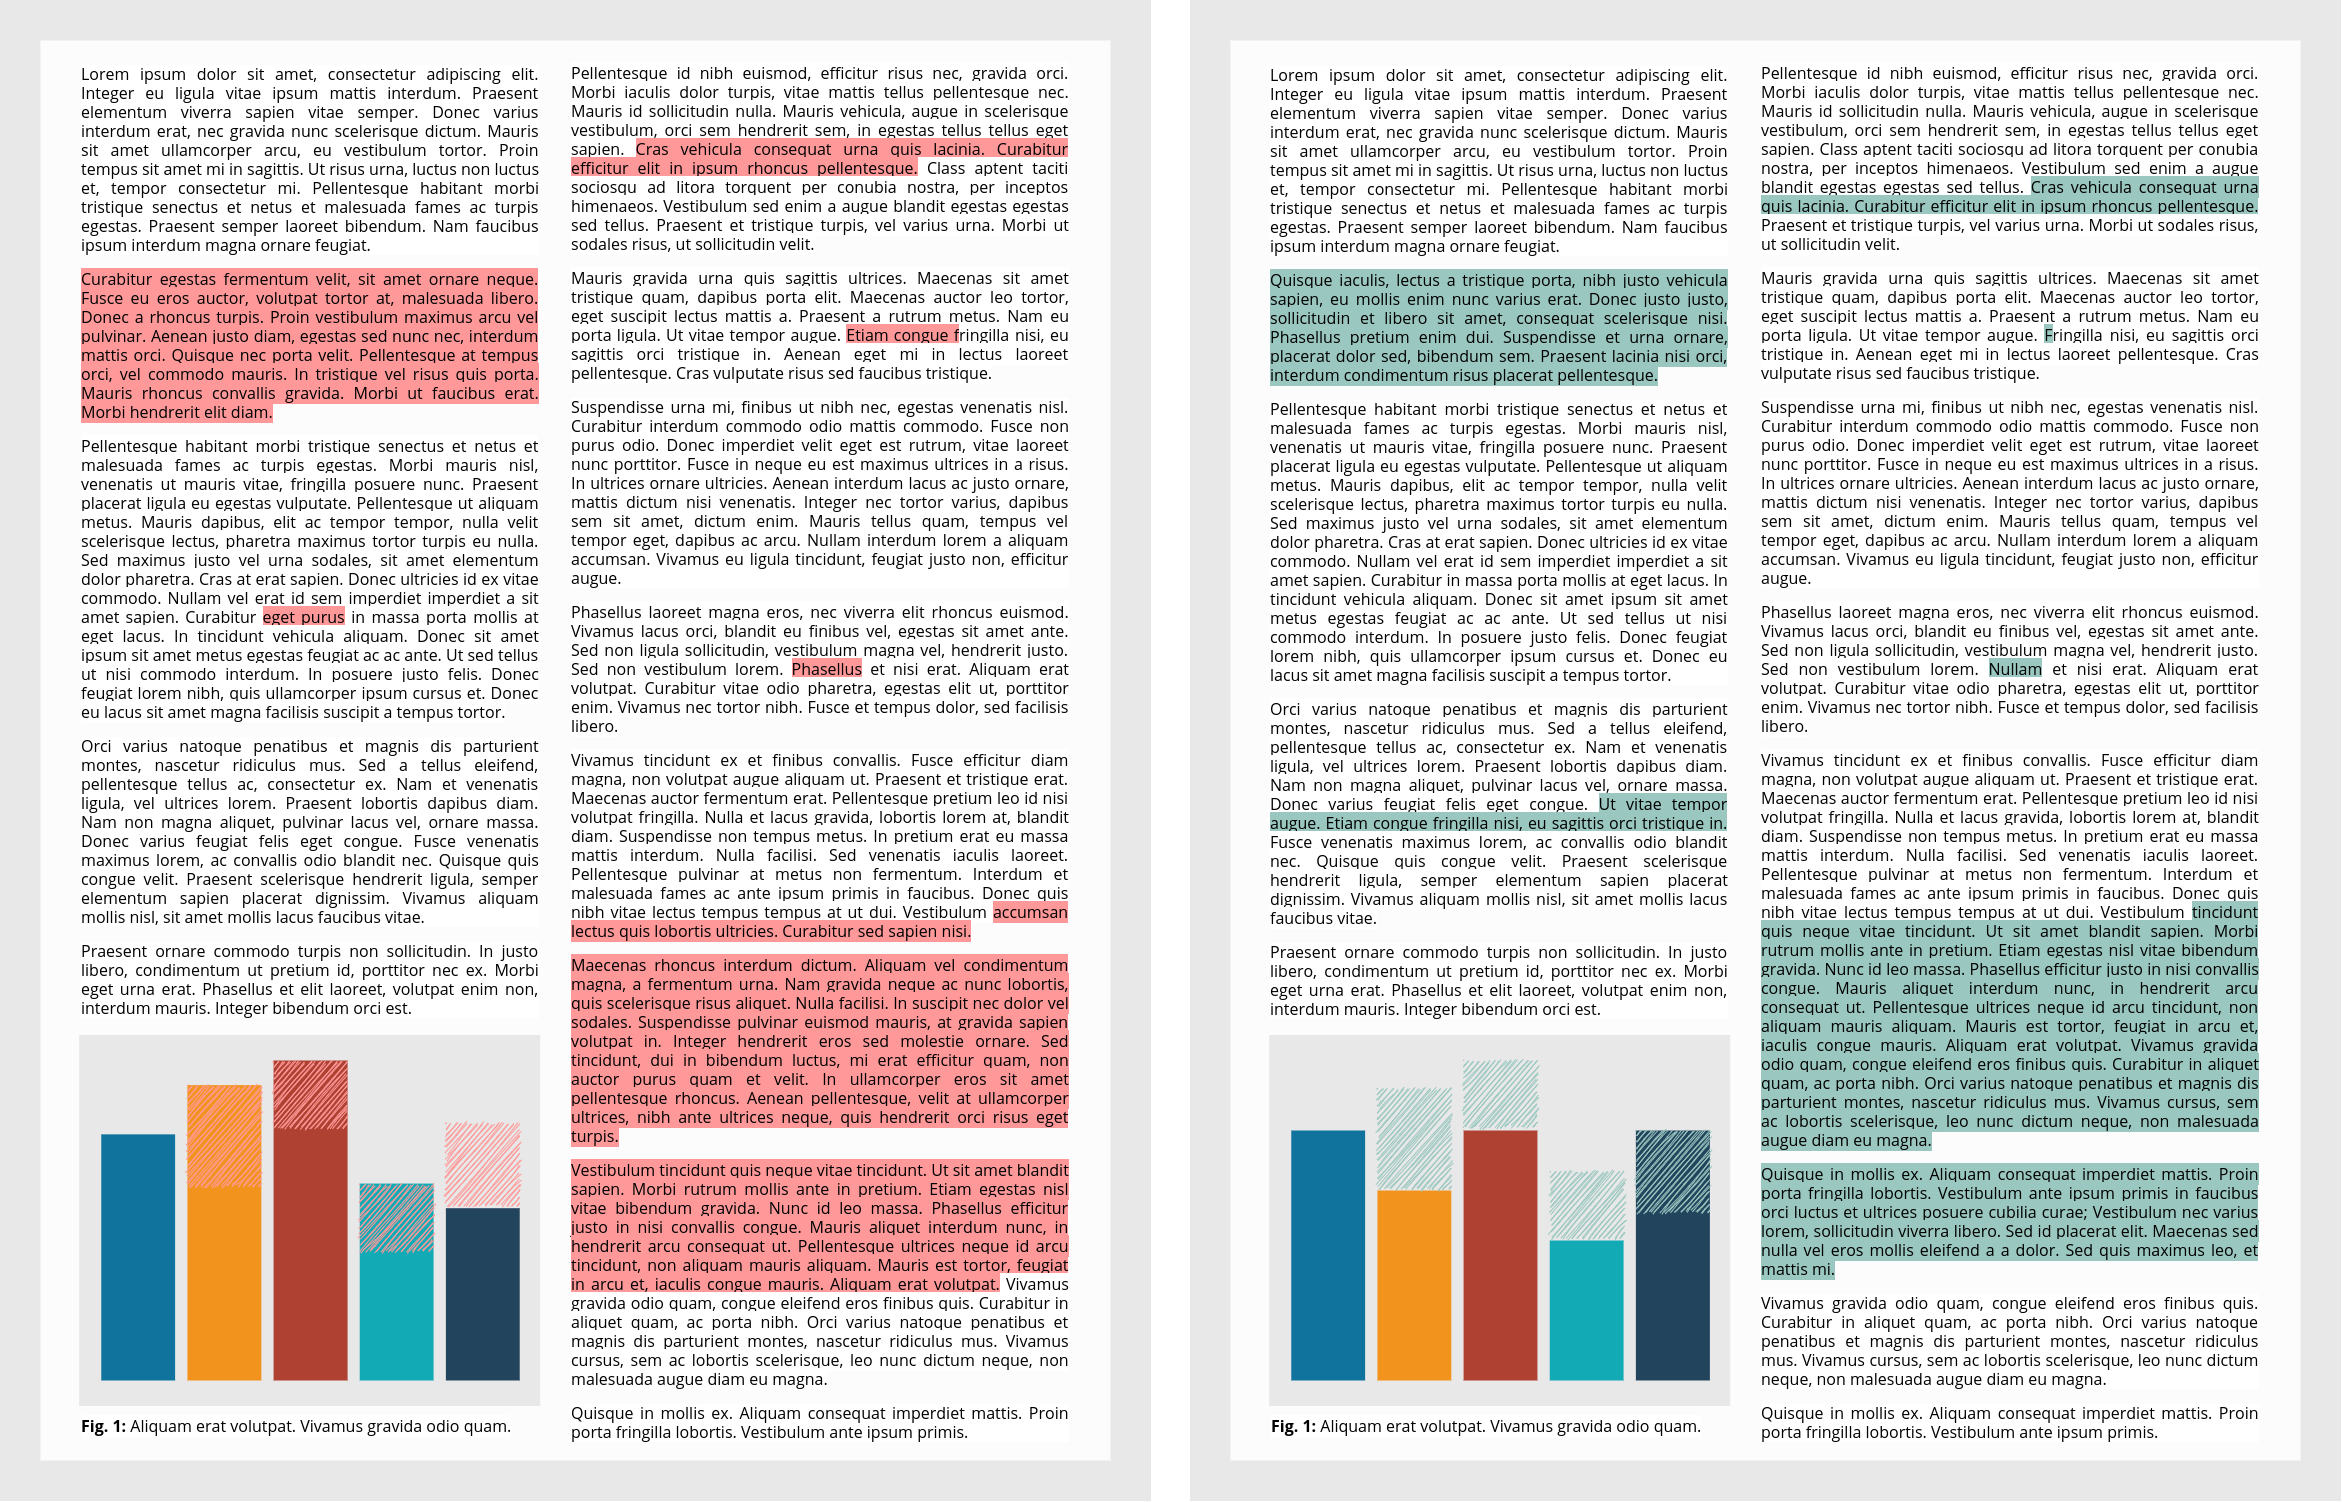
\includegraphics[width=0.48\textwidth]{figures/paper-pdf-delta.png}
    \caption{Detailed visual comparison report (mock-up); left shows what has been removed in the previous version's PDF, right shows what has been added to the latest version's PDF.}
    \label{fig:paper-pdf-delta}
\end{figure}

%%%%%%%%%%%%%%%%%%%%%%%%%%%%%%%%%%%%%%%%%%%%
%%%%%%%%%%%%%%%%%%%%%%%%%%%%%%%%%%%%%%%%%%%%
%%%%%%%%%%%%%%%%%%%%%%%%%%%%%%%%%%%%%%%%%%%%
%%%%%%%%%%%%%%%%%%%%%%%%%%%%%%%%%%%%%%%%%%%%
%%%%%%%%%%%%%%%%%%%%%%%%%%%%%%%%%%%%%%%%%%%%

\clearpage

\begin{table*}[b]
    \centering
    \caption{NSDI '20 analysis overview ordered by program appearance.}\vspace{3pt}
    \begin{tabular}{| C{0.55cm} | C{0.65cm} || C{0.9cm} | C{0.8cm} | C{0.95cm} | C{1.1cm} | C{0.5cm} | } \hline
        \textbf{\#} & \textbf{Ref.} & \textbf{Tweak} & \textbf{C/S/E} & \textbf{Cloud} & \textbf{Custom} & \textbf{DS} \\ \hline
%%%%%%%%%%%%%%%%%%%%%%%%%%%%%%
1 & \cite{nsdi-2020-mellette} & \checkmark & \checkmark &  & \checkmark &  \\ \hline
2 & \cite{nsdi-2020-cheng} & \checkmark & \checkmark &  & \checkmark &  \\ \hline
3 & \cite{nsdi-2020-jha} &  &  &  & \checkmark & \checkmark \\ \hline
4 & \cite{nsdi-2020-alcoz} & \checkmark & \checkmark &  & \checkmark &  \\ \hline
5 & \cite{nsdi-2020-moon} & \checkmark &  &  & \checkmark &  \\ \hline
6 & \cite{nsdi-2020-arashloo} & \checkmark & \checkmark &  & \checkmark &  \\ \hline
7 & \cite{nsdi-2020-yang} & \checkmark &  &  & \checkmark &  \\ \hline
8 & \cite{nsdi-2020-hwang} & \checkmark &  &  & \checkmark &  \\ \hline
9 & \cite{nsdi-2020-kuga} & \checkmark &  &  & \checkmark &  \\ \hline
10 & \cite{nsdi-2020-uluyol} & \checkmark &  & \checkmark &  &  \\ \hline
11 & \cite{nsdi-2020-yuan} &  & \checkmark & \checkmark &  &  \\ \hline
12 & \cite{nsdi-2020-abhashkumar} &  & \checkmark &  &  &  \\ \hline
13 & \cite{nsdi-2020-zhang-kaiyuan} &  & \checkmark &  & \checkmark &  \\ \hline
14 & \cite{nsdi-2020-zhang-peng} &  & \checkmark &  &  &  \\ \hline
15 & \cite{nsdi-2020-yousefi} &  & \checkmark &  &  &  \\ \hline
16 & \cite{nsdi-2020-lai} & \checkmark &  & \checkmark &  &  \\ \hline
17 & \cite{nsdi-2020-mahajan} & \checkmark & \checkmark & \checkmark &  &  \\ \hline
18 & \cite{nsdi-2020-liu-ming} & \checkmark &  &  & \checkmark &  \\ \hline
19 & \cite{nsdi-2020-ding} & \checkmark & \checkmark & \checkmark &  &  \\ \hline
20 & \cite{nsdi-2020-gadre} &  &  &  & \checkmark &  \\ \hline
21 & \cite{nsdi-2020-goyal} & \checkmark & \checkmark &  & \checkmark &  \\ \hline
22 & \cite{nsdi-2020-carver} &  &  &  & \checkmark &  \\ \hline
23 & \cite{nsdi-2020-li} & \checkmark &  &  & \checkmark &  \\ \hline
24 & \cite{nsdi-2020-mogul} &  &  &  &  &  \\ \hline
25 & \cite{nsdi-2020-agache} & \checkmark &  & \checkmark &  &  \\ \hline
26 & \cite{nsdi-2020-mehta} &  &  &  & \checkmark &  \\ \hline
27 & \cite{nsdi-2020-vuppalapati} &  &  &  & \checkmark & \checkmark \\ \hline
28 & \cite{nsdi-2020-brooker} & \checkmark & \checkmark &  & \checkmark &  \\ \hline
29 & \cite{nsdi-2020-vermeulen} &  &  & \checkmark &  & \checkmark \\ \hline
30 & \cite{nsdi-2020-yan} & \checkmark &  & \checkmark & \checkmark &  \\ \hline
31 & \cite{nsdi-2020-uta} & \checkmark &  & \checkmark &  &  \\ \hline
32 & \cite{nsdi-2020-song} & \checkmark & \checkmark & \checkmark &  &  \\ \hline
33 & \cite{nsdi-2020-hauer} &  &  &  & \checkmark &  \\ \hline
34 & \cite{nsdi-2020-lou} & \checkmark &  & \checkmark &  &  \\ \hline
%%%%%%%%%%%%%%%%%%%%%%%%%%%%%%
    \end{tabular}
    \hspace{0.2cm}
    \begin{tabular}{| C{0.55cm} | C{0.65cm} || C{0.9cm} | C{0.8cm} | C{0.95cm} | C{1.1cm} | C{0.5cm} | } \hline
        \textbf{\#} & \textbf{Ref.} & \textbf{Tweak} & \textbf{C/S/E} & \textbf{Cloud} & \textbf{Custom} & \textbf{DS} \\ \hline
%%%%%%%%%%%%%%%%%%%%%%%%%%%%%%
35 & \cite{nsdi-2020-zhai} & \checkmark &  &  & \checkmark &  \\ \hline
36 & \cite{nsdi-2020-burke} & \checkmark &  & \checkmark &  &  \\ \hline
37 & \cite{nsdi-2020-hu-jiyao} & \checkmark & \checkmark &  &  & \checkmark \\ \hline
38 & \cite{nsdi-2020-levai} & \checkmark &  &  & \checkmark &  \\ \hline
39 & \cite{nsdi-2020-mukerjee} & \checkmark &  & \checkmark & \checkmark &  \\ \hline
40 & \cite{nsdi-2020-barbette} & \checkmark &  &  & \checkmark &  \\ \hline
41 & \cite{nsdi-2020-sharma} & \checkmark & \checkmark &  & \checkmark &  \\ \hline
42 & \cite{nsdi-2020-hsu} & \checkmark & \checkmark & \checkmark &  &  \\ \hline
43 & \cite{nsdi-2020-takruri} & \checkmark &  &  & \checkmark &  \\ \hline
44 & \cite{nsdi-2020-pouryousef} & \checkmark &  & \checkmark &  &  \\ \hline
45 & \cite{nsdi-2020-kwon} & \checkmark &  & \checkmark &  &  \\ \hline
46 & \cite{nsdi-2020-sivaraman} & \checkmark & \checkmark &  &  &  \\ \hline
47 & \cite{nsdi-2020-arzani} & \checkmark &  &  & \checkmark & \checkmark \\ \hline
48 & \cite{nsdi-2020-hunt} & \checkmark & \checkmark & \checkmark &  &  \\ \hline
49 & \cite{nsdi-2020-burkhalter} & \checkmark &  & \checkmark & \checkmark &  \\ \hline
50 & \cite{nsdi-2020-hu-yuncong} & \checkmark &  & \checkmark &  &  \\ \hline
51 & \cite{nsdi-2020-mardani} &  &  &  & \checkmark &  \\ \hline
52 & \cite{nsdi-2020-liu-xin} &  &  &  & \checkmark &  \\ \hline
53 & \cite{nsdi-2020-kumar} &  &  &  & \checkmark &  \\ \hline
54 & \cite{nsdi-2020-zhao} &  &  &  & \checkmark &  \\ \hline
55 & \cite{nsdi-2020-prabhu} &  & \checkmark &  &  &  \\ \hline
56 & \cite{nsdi-2020-birkner} &  & \checkmark &  &  &  \\ \hline
57 & \cite{nsdi-2020-burnett} &  &  &  & \checkmark &  \\ \hline
58 & \cite{nsdi-2020-kakarla} &  & \checkmark &  &  &  \\ \hline
59 & \cite{nsdi-2020-yaseen} & \checkmark &  &  & \checkmark &  \\ \hline
60 & \cite{nsdi-2020-hessar} &  &  &  & \checkmark &  \\ \hline
61 & \cite{nsdi-2020-arun} &  &  &  & \checkmark &  \\ \hline
62 & \cite{nsdi-2020-ahmad} &  & \checkmark &  & \checkmark &  \\ \hline
63 & \cite{nsdi-2020-ha} &  &  &  & \checkmark &  \\ \hline
64 & \cite{nsdi-2020-chen} &  &  &  & \checkmark &  \\ \hline
65 & \cite{nsdi-2020-ayyalasomayajula} &  &  &  & \checkmark &  \\ \hline
%%%%%%%%%%%%%%%%%%%%%%%%%%%%%%
 &  &  &  &  &  & \\ \hline
 \multicolumn{2}{| c ||}{\textbf{Total}} & \textbf{38} & \textbf{23} & \textbf{19} & \textbf{40} & \textbf{5} \\ \hline
 \multicolumn{2}{| c ||}{\textbf{Fraction}} & \textbf{58\%} & \textbf{35\%} & \textbf{29\%} & \textbf{62\%} & \textbf{8\%} \\ \hline
    \end{tabular}
\label{tab:nsdi2020}
\end{table*}

\section{NSDI 2020 analysis}
\label{appendix:nsdianalysis}

In order to assess the applicability of \sysname, we went through the 65 papers of NSDI 2020. For each paper we registered the following characteristics:

\begin{itemize}[leftmargin=10pt,itemsep=2pt,topsep=2pt]

    \item \textbf{Tweak:} Whether we could identify experimental setup parameters which could be of interest for the reader to tweak with \sysname. Certain types of work are \textbf{excluded} even though they may have parameters or configurations of interest:
    
    \begin{itemize}[leftmargin=10pt,itemsep=2pt,topsep=2pt]
        \item Predominantly measurement studies
        \item Custom hardware wireless communication systems in the physical world (as setup involves physical steps)
        \item Verification systems (as the outcome is typically binary)
        \item Operational experience studies
    \end{itemize}

    \item \textbf{C/S/E:} The presence of experiments aimed to be run over general compute: \textbf{C}alculation, \textbf{S}imulation or \textbf{E}mulation. This excludes emulated deployments of the system on external cloud infrastructure as they fall into the next category.
    
    \item \textbf{Cloud:} The presence of explicit system deployment experiments using publicly accessible (cloud) infrastructure (\eg PlanetLab, Emulab, AWS, Azure, Google Cloud).
    
    \item \textbf{Custom:} The presence of experiments using custom hardware (\eg custom chips) or non-public infrastructure.
    
    \item \textbf{Dataset (DS):} The paper explicitly showcases a dataset. (We do not check for public availability of the dataset.)
    
\end{itemize}

\noindent When in doubt, \eg for research problems we have less familiarity with, we leaned towards a conservative analysis, \eg not checking the box for interesting parameters to tweak, if we were unsure. The results are displayed in Table~\ref{tab:nsdi2020}.

%%%%%%%%%%%%%%%%%%%%%%%%%%%%%%%%%%%%%%%%%%%%
%%%%%%%%%%%%%%%%%%%%%%%%%%%%%%%%%%%%%%%%%%%%
%%%%%%%%%%%%%%%%%%%%%%%%%%%%%%%%%%%%%%%%%%%%
%%%%%%%%%%%%%%%%%%%%%%%%%%%%%%%%%%%%%%%%%%%%
%%%%%%%%%%%%%%%%%%%%%%%%%%%%%%%%%%%%%%%%%%%%

\clearpage
\section{Replication instructions}

Below we detail the replication instructions. It assumes Ubuntu LTE 18.04, 20.04 or later, and Python version 3.7 or higher (with \texttt{pip} installed). Additional information can be found in the \texttt{README.md} of the code repository.

\begin{enumerate}
    \item Clone (or download from the venue website) the code repository and navigate into it:\\
    \\
    \texttt{git clone https://github.com/snkas/codebind-paper.git}\\
    \texttt{cd codebind-paper}\\

    \item Setup environment (\ie install dependencies) (duration: $\pm$8~min.):\\
    \\
    \texttt{bash setup\_env.sh}\\

    \item (\textit{Optional}) It takes quite some time for the next step (reproduce) to rerun all experiments, as such for convenience an archive with the runs already finished is provided:\\
    \\
    \texttt{mkdir -p temp}\\
    \texttt{tar -xzf partial-temp-runs.tar.gz -C temp}\\
    \\
    Skip this step if you wish to replicate from scratch.\\

    \item Reproduce the paper (duration: $\pm$8~hours without optional extraction, $\pm$15-20~min. with):\\
    \\
    \texttt{bash reproduce.sh}\\

    \item The paper is output at: \texttt{paper-latex/out/paper.pdf}\\

\end{enumerate}

\noindent We also provide a short (5:31) video demonstration of the process (please set quality manually to 720p):\\

\noindent\url{https://drive.google.com/file/d/1f8gu3MpWzXM4WbpFLy7DXDcR4z3s6Ws9/view}\\

\noindent \textit{The code repository makes use of ns-3~\cite{ns3}, the basic-sim ns-3 module \cite{basic-sim}, top-lists~\cite{top-lists}, ACM LaTeX class files~\cite{acm-latex}, and several gnuplot files. See the complete license at ./LICENSE for more detailed information. It moreover makes use of several distribution packages (texlive~\cite{texlive}, gnuplot~\cite{gnuplot}, openmpi~\cite{openmpi}, lcov~\cite{lcov}) and Python modules (texsoup~\cite{texsoup}, exputilpy~\cite{exputilpy}, networkx~\cite{networkx}, matplotlib~\cite{matplotlib}, pandas~\cite{pandas}, numpy~\cite{numpy}, statsmodels~\cite{statsmodels}).}
